\documentclass[12pt]{article}
\usepackage[all, stdclass]{lix}
\usepackage{graphicx}
\usepackage{svg}
\usepackage{pgfplots}
\svgsetup{
  inkscapepath=assets/,  % Path to the directory containing your SVG files
  svgpath=assets/        % Path to the directory containing your SVG files
}
\usepackage{float}
\usepackage{hyperref}
\usepackage{url}
\usepackage{times}
\usepackage{amsmath}
\usepackage{enumitem}
\usepackage{subcaption}
\usepackage{tikz}
\setlist{topsep=0pt, leftmargin=*}
%----------EDIT COVER INFO HERE -----------------%
\def \LOGOPATH {assets/birzeit-logo.png}
\def \DEPARTEMENT {Department of Electrical \& Computer Engineering}
\def \COURSENUM {ENEE4113}
\def \COURSENAME {Communications Laboratory}
\def \REPORTTITLE {Frequency Modulation}
\def \STUDENTNAME {Mohammad Abu-Shelbaia}
\def \STUDENTID {1200198}
\def \INSTRUCTOR {Dr. Ibrahim Nemer}
\def \ASSISTANT {Eng. Mohammad Al-Battat}
\def \REPORTNUM {4}

\begin{document}
\pagenumbering{Roman}

\begin{titlepage}
    \vfill
    \begin{center}
        \includegraphics[width=0.7\textwidth]{\LOGOPATH} \\
        \hfill \\
        \Large{\DEPARTEMENT} \\
        \Large{\COURSENUM\;-\;\COURSENAME} \\
        \vfill
        \textbf{\LARGE{Experiment \#\REPORTNUM}} \\
        \textbf{\LARGE{\REPORTTITLE}}
    \end{center}
    \vfill
    \begin{flushleft}
        \Large{\textbf{Prepared by:}\\ \STUDENTNAME\quad\STUDENTID} \\

        \Large{\textbf{Instructor:} \INSTRUCTOR} \\
        \Large{\textbf{Assistant:} \ASSISTANT} \\
        \Large{\textbf{Section:} 4}\\
        \LARGE{\textbf{ }}\\
        \LARGE{\textbf{ }}\\
        \LARGE{\textbf{ }}\\
        \Large{\textbf{Date:} \today}\\
    \end{flushleft}
    \vfill
\end{titlepage}


%--------------- TABLES --------------------------------%
\tableofcontents
\clearpage
\setlength{\parskip}{\baselineskip}%
\listoffigures
\clearpage
\listoftables
\clearpage
\pagenumbering{arabic}
%-------------- CONTENT ---------------------%
\h{Theory}
\hh{Modulation Scheme}
Frequency modulation is a part of angle modulation, angle modulation is a technique with constant carrier amplitude and varying phase or time derivative of phase. an FM signal can be expressed as:
\begin{equation}
    s(t) = A_c \cos({\omega}_c t + 2\pi k_f\int_{-\infty}^{t}m(\tau)\,d\tau)
\end{equation}
\begin{itemize}
    \item $A_c$ is the carrier amplitude
    \item ${\omega}_c$ is the carrier frequency
    \item $k_f$ is the modulation sensitivity
    \item $m(t)$ is the message signal
\end{itemize}
\begin{figure}[H]
    \centering
    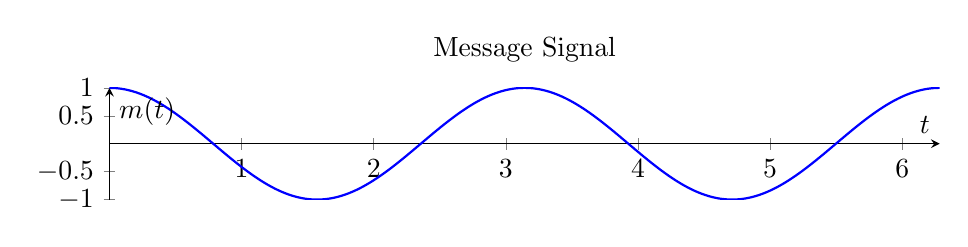
\begin{tikzpicture}
        \begin{axis}[
            width=1\textwidth,
            height=3cm,
            xlabel={$t$},
            ylabel={$m(t)$},
            domain=0:2*pi,
            samples=500,
            axis lines=middle,
            title={Message Signal},
            legend style={at={(0.5,-0.3)},anchor=north},
        ]
        \addplot[blue, thick] {cos(deg(2*x))};
        \end{axis}
    \end{tikzpicture}
    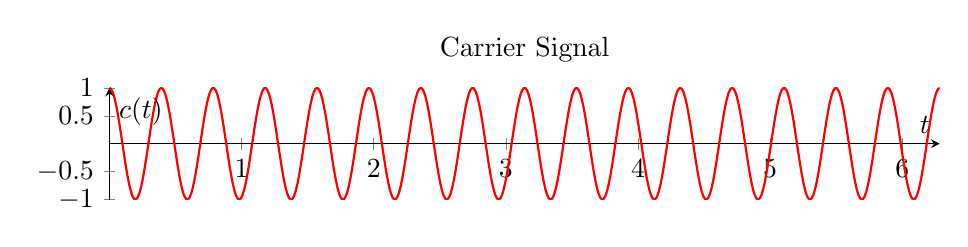
\begin{tikzpicture}
    \begin{axis}[
        width=1\textwidth,
        height=3cm,
        xlabel={$t$},
        ylabel={$c(t)$},
        domain=0:2*pi,
        samples=500,
        axis lines=middle,
        title={Carrier Signal},
        legend style={at={(0.5,-0.3)},anchor=north},
    ]
    \addplot[red, thick] {cos(deg(16*x))};
    \end{axis}
    \end{tikzpicture}
    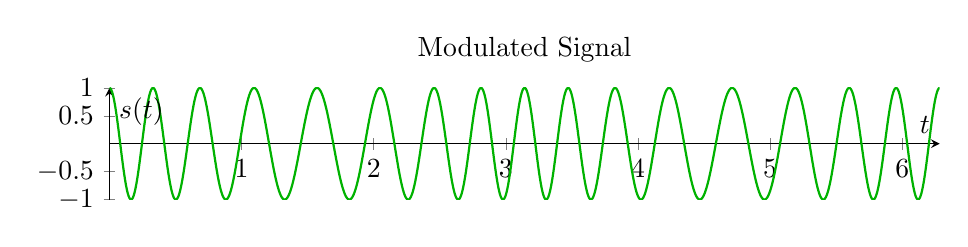
\begin{tikzpicture}
        \begin{axis}[
            width=1\textwidth,
            height=3cm,
            xlabel={$t$},
            ylabel={$s(t)$},
            domain=0:2*pi,
            samples=1000,
            axis lines=middle,
            title={Modulated Signal},
            legend style={at={(0.5,-0.2)},anchor=north},
        ]
        \addplot[green!70!black, thick] {cos(deg(16*x) + 2*pi*15*sin(deg(2*x)))}; % fc = 1, Kf = 64
        \end{axis}
        \end{tikzpicture}
    \caption{Frequency Modulation Scheme}
\end{figure}
\hhh{Modulation}
There are two types of modulation, narrowband and wideband. narrowband modulation is when the modulation index is less than 1, and wideband modulation is when the modulation index is greater than 1. The modulation index is defined as:
\begin{equation}
    \beta = \frac{\Delta f}{f_m} = \frac{k_f A_m}{f_m}
\end{equation}
The simplest way of generating an FM signal is using a voltage-controlled oscillator, which is not a stable method. the other method is generating a narrowband FM signal and then using a frequency multiplier to generate a wideband FM signal.

\begin{figure}[H]
    \centering
    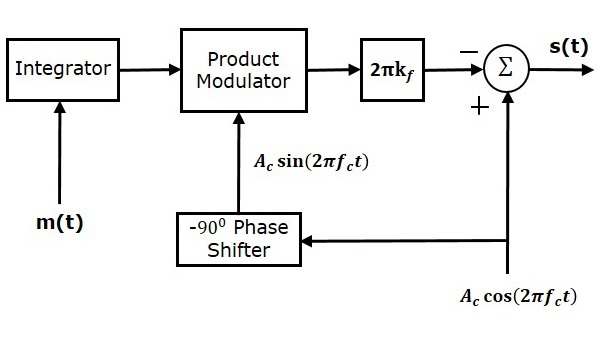
\includegraphics[width=0.5\textwidth]{assets/img/nbfm_modulator.jpg}
    \caption{Narrowband FM Generation}
    \cite{tutorialspoint_fm_modulators}
\end{figure}
\begin{figure}[H]
    \centering
    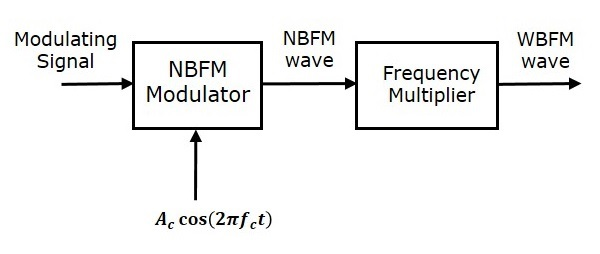
\includegraphics[width=0.5\textwidth]{assets/img/indirect_method.jpg}
    \caption{Wideband FM Generation}
    \cite{tutorialspoint_fm_modulators}
\end{figure}
\hhh{Demodulation - Phase Locked Loop}
For demodulation, a common method is the phase-locked loop (PLL) a feedback system that synchronizes the phase of the output signal with the phase of the input signal. The phase detector compares the phase of the input signal with the phase of the output signal and generates an error signal that is used to adjust the phase of the output signal. The output of the phase detector is filtered using a low-pass filter to remove high-frequency components, resulting in a demodulated signal.
\begin{figure}[H]
    \centering
    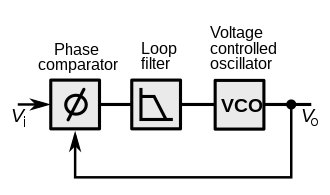
\includegraphics[width=0.5\textwidth]{assets/img/PLL.png}
    \caption{Phase Locked Loop}
    \cite{wikipedia_pll}
\end{figure}
\hh{Carson's Rule}
Carson's rule is a rule of thumb that gives the approximate bandwidth of an FM signal. It states that A 98\% power B.W of an FM signal can be estimated by:

\begin{equation}
    B_T \approx 2(\beta + 1)f_m
\end{equation}
The rule works well when the message signal is continuous. However, it cannot be used when the message contains discontinuities, such as in the case of a square function. \cite{tutorialspoint_fm_modulators}
\hh{Besel Functions}
A more accurate expression for the FM signal bandwidth can be obtained using Bessel functions. The FM signal can be expressed as:
\begin{equation}
    s(t) = A_c \cos({\omega}_c t + \beta\sin({\omega}_m t))
\end{equation} 
where $\beta$ is the modulation index, and ${\omega}_m$ is the message signal frequency. In terms of Bessel functions, the FM signal can be expressed as:
\begin{equation}
    s(t) = A_c \sum_{n=-\infty}^{\infty} J_n(\beta) \cos({\omega}_c t + n{\omega}_m t)
\end{equation}
In order to find the bandwidth of the FM signal that achieves a certain percentage of the total power, the following equation can be used:
\begin{equation}
    J_0^{2}(\beta) + 2\sum_{n=1}^{m} J_n^{2}(\beta) = p
\end{equation}
where $p$ is the percentage of the total power, and $m$ is the number of Bessel functions to be summed, the bandwidth of the FM signal can be calculated using:
\begin{equation}
    B_T = 2*m*f_m
\end{equation}
\hh{Zero Crossing Decay}
Zero Crossing is a method to get rid of the carrier spectra,
and since the spectral components are proportional to the Bessel functions, the zero crossing of the carrier signal occurs when the Bessel function is zero $J_0(\beta) = 0$. 
\clearpage
\h{Procedure and Data Analysis}
\hh{Modulation}
\hhh{Time Domain}
\begin{figure}[H]
    \centering
    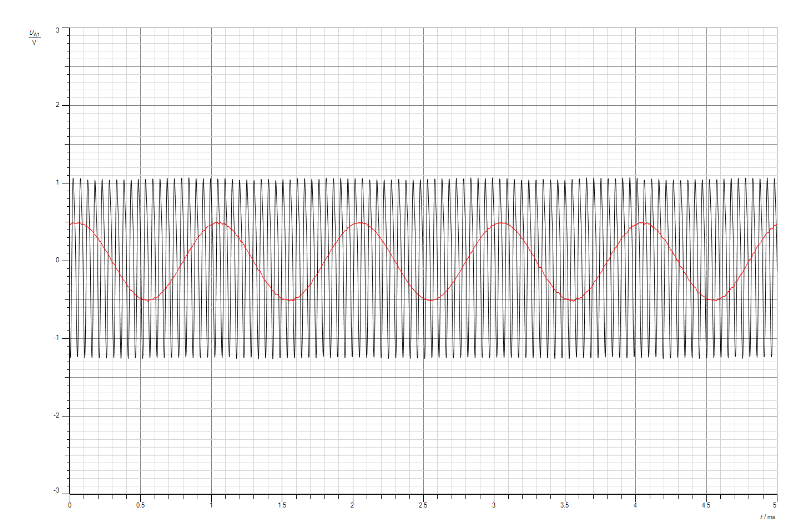
\includegraphics[width=0.5\textwidth]{assets/time_domain.png}
    \caption{Time Domain}
\end{figure}
\hhh{Frequency Domain}
\begin{figure}[H]
    \centering
    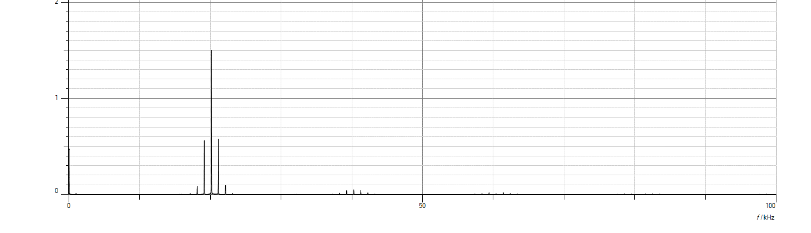
\includegraphics[width=1\textwidth]{assets/freqeuncy_domain.png}
    \caption{Frequency Domain}
\end{figure}
The modulated signal isn't affected by the amplitude of the message signal, but the frequency of the message signal affects the frequency of the modulated signal.
\hhh{Setting Carrier Frequency}
In order to set the carrier frequency to 20kHz, we set the message signal to 0, so the modulated signal is just the carrier signal.
\begin{equation}
    \begin{aligned}
        s(t) &= A_c \cos({\omega}_c t + \beta\int_{0}^{t} m(\tau) d\tau) \\
        s(t) &= A_c \cos({\omega}_c t + \beta\times 0)\\
        s(t) &= A_c \cos({\omega}_c t)
    \end{aligned}
\end{equation}
\begin{figure}[H]
    \centering
    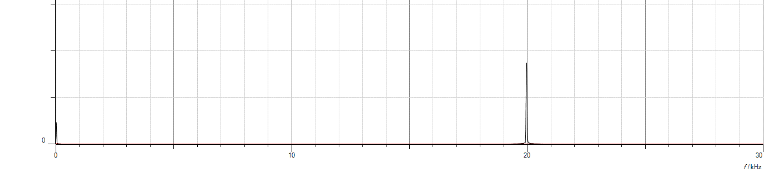
\includegraphics[width=1\textwidth]{assets/carrier.png}
    \caption{Carrier Frequency}
\end{figure}
from the classy lab sample, we can see that the carrier frequency is 19.91kHz, which is close to 20kHz.
\hhh{Characteristics of the FM Modulator}
The main Characteristic of the FM modulator is the modulation sensitivity $K_f$, using the instantaneous frequency equation:
\begin{equation}
    f_i = f_c + k_f m(t)
\end{equation}
using a constant amplitude would result
\begin{equation}
    f_i = f_c + k_f \times A_m
\end{equation}
with $f_c$ being the carrier frequency, $k_f$ being the modulation sensetivity, and $A_m$ being the amplitude of the message signal. 
\begin{table}[H]
    \centering
    \begin{tabular}{l|r|r|r|r|r|r|r|r|r|r|r}
    \hline
    Voltage  & -10   & -8   & -6    & -4    & -2    & 0     & 2     & 4  & 6     & 8     & 10 \\ \hline
    Frequency & 19.06 & 19.2 & 19.32 & 19.45 & 19.59 & 19.73 & 19.85 & 20 & 20.13 & 20.26 & 20.39 \\ \hline
    \end{tabular}
    \caption{Carrier Frequency vs Message Voltage - $k_f$}
\end{table}

\begin{figure}[H]
    \centering
    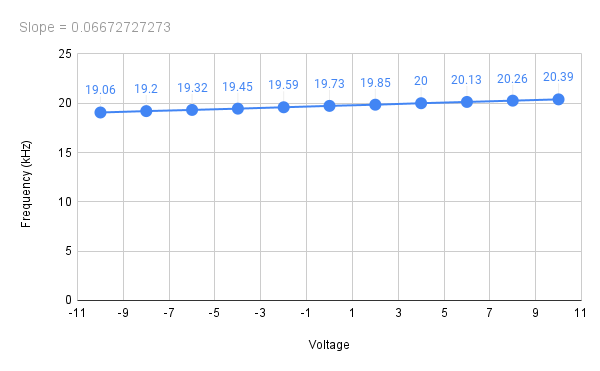
\includegraphics[width=1\textwidth]{assets/img/chart.png}
    \caption{Carrier Frequency vs Message Voltage - $k_f$}
\end{figure}
the slope of the graph is the modulation sensetivity $k_f$, which is 66.6 Hz/V.
For a 10V message signal, the maximum frequency deviation is given by:
\begin{equation}
    \begin{aligned}
        \Delta f &= k_f \times A_m = 66.6 \times 10 = 666 Hz
    \end{aligned}
\end{equation}
\hhh{FM signal spectrum for different message signals}
In this part, we used a 10V sinusoidal message signal with two frequencies 3kHz, and 200Hz.
\begin{figure}[H]
    \centering
    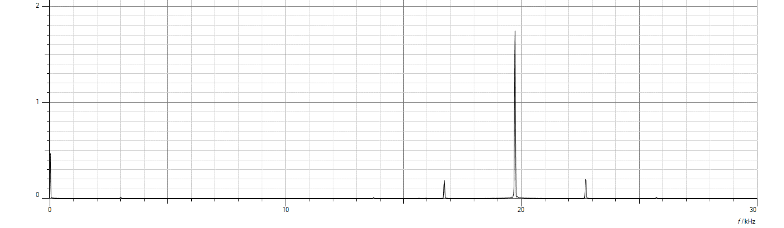
\includegraphics[width=1\textwidth]{assets/3k.png}
    \caption{S(F) - 3kHz Message Signal}
\end{figure}
\begin{figure}[H]
    \centering
    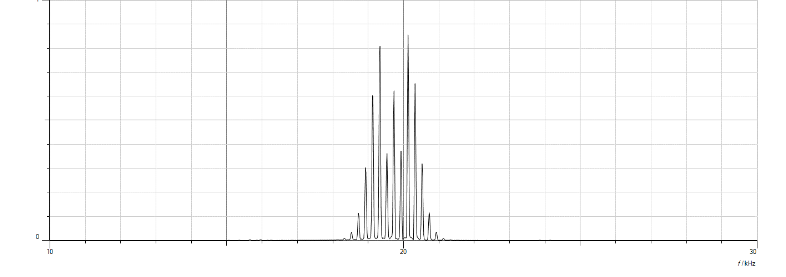
\includegraphics[width=1\textwidth]{assets/200.png}
    \caption{S(F) - 200Hz Message Signal}
\end{figure}
We notice that the density of the spectrum is higher for the 200Hz message signal, this is because the spectra are 3kHz apart in the first case, and 200Hz apart in the second case.\\
for a square message signal, with 200Hz frequency, 0.5 duty cycle, and 10V the spectrum is as follows:
\begin{figure}[H]
    \centering
    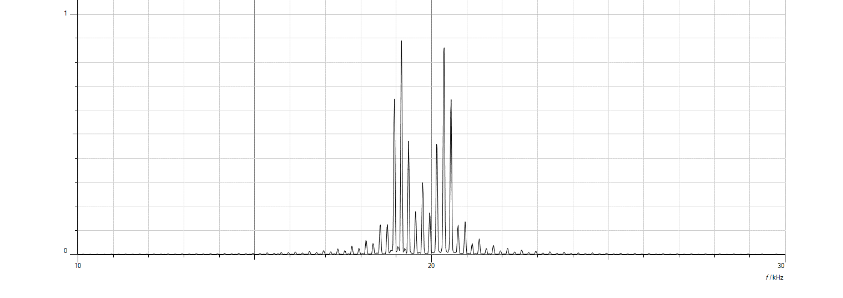
\includegraphics[width=1\textwidth]{assets/square.png}
    \caption{S(F) - Square Message Signal}
\end{figure}
We noticed that the spectrum is similar to the spectrum of the 200Hz sinusoidal message signal, but the density of the spectrum is higher, this is because the square wave has more harmonics than the sinusoidal wave.
\hhh{Zero Carrier Crossing}
Since the spectral components are proportional to the Bessel functions, the zero crossing of the carrier signal occurs when the Bessel function is zero. The first three values for $\beta$ that satisfy this condition are 2.4048, 5.5201, and 8.6537. For a constant frequency of 100Hz, the corresponding amplitudes can be calculated as follows:
\begin{equation}
    \beta = {K_f \times A_m \over f_m}
    \label{HI}
\end{equation}
\begin{table}[H]
    \centering

    \begin{tabular}{l|r|r|r}
        \hline
        $\beta$ & 2.4048 & 5.5201 & 8.6537 \\\hline
        $A_m$ & 3.643 & 8.363 & 13.111 \\\hline
    \end{tabular}
    \caption{Amplitude zero crossing values}
\end{table}
experimentally, we found the first decay at 7.3 VSS, which means $A_M$ = 3.65, which is close to the theoretical value.
\begin{figure}[H]
    \centering
    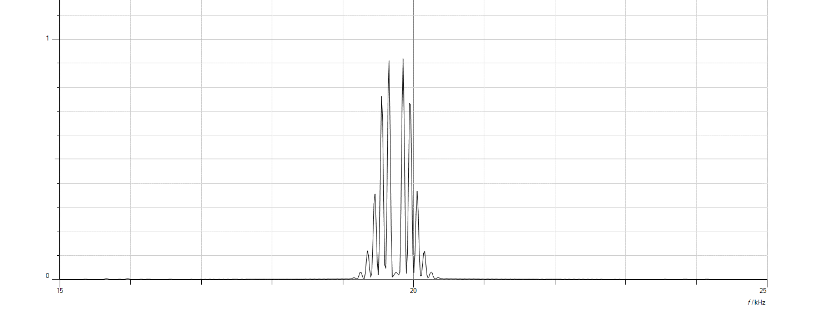
\includegraphics[width=0.7\textwidth]{assets/decay_1.png}
    \caption{First Amplitude Zero Crossing Decay}
\end{figure}
Another way of finding the first zero crossing is to use a constant amplitude and vary the frequency. Using (Equation\ref{HI}) and a constant 10V amplitude we can fill the following table:
\begin{table}[H]
    \centering
    \begin{tabular}{l|r|r|r}
        \hline
        $\beta$ & 2.4048 & 5.5201 & 8.6537 \\\hline
        Frequency & 276.94 & 120.65 & 76.96 \\\hline
    \end{tabular}
    \caption{Amplitude zero crossing values}
\end{table}
experimentally, we found that decay at 280kHz is not nessecarly the first decay since we didn't check for smaller values.
\begin{figure}[H]
    \centering
    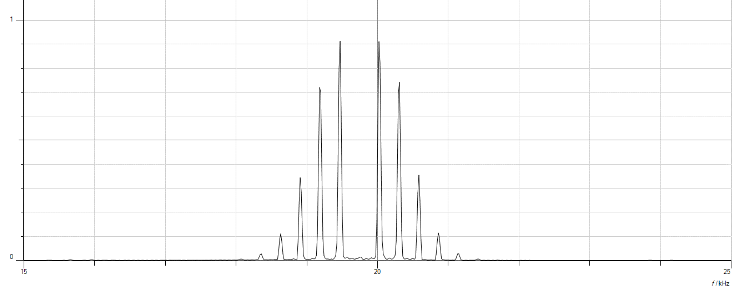
\includegraphics[width=0.9\textwidth]{assets/decay_2.png}
    \caption{Frequency Zero Crossing Decay}
\end{figure}
\hh{Demodulation}
\hhh{Demodulated Signal}
Setting Vss = 10 V and $f_m$ = 500 Hz and using demodulator $\tau_2$ filter, we were able to recover the message using PLL demodulation as shown in the following figures:
\begin{figure}[H] 
    \centering
    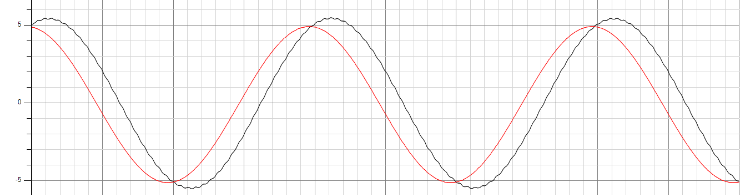
\includegraphics[width=1\textwidth]{assets/d_t.png}
    \caption{Demodulated Signal in the time domain}
\end{figure}
\begin{figure}[H] 
    \centering
    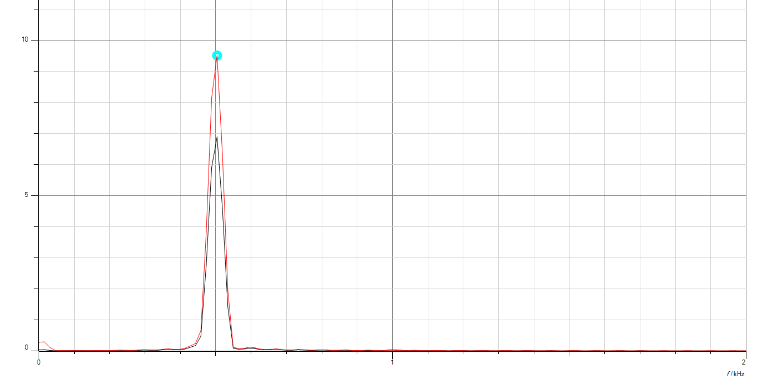
\includegraphics[width=1\textwidth]{assets/d_f.png}
    \caption{Demodulated Signal in the frequency domain}
\end{figure}
\hhh{Loop Filter Effect}
for a message signal with 4V amplitude and 500Hz frequency, we used two different loop filters, $\tau_1$ and $\tau_2$, and we measured the amplitude of the demodulated signal for different message frequencies and the results are as follows:
\begin{table}[H]
    \centering
    \begin{tabular}{|r|r|r|}
    \cline{1-3}
    \multicolumn{1}{|l|}{Frequency} & \multicolumn{1}{l|}{$A_D$ using $\tau_1$} & \multicolumn{1}{l|}{$A_D$ using $\tau_2$} \\
    \cline{1-3}
    500  & 8.9  & 2.75 \\
    1000 & 4.31 & 2.57 \\
    1500 & 2.93 & 2.55 \\
    2000 & 2.1  & 2.25 \\
    3000 & 1.19 & 1.45 \\
    4000 & 0.81 & 0.96 \\
    \cline{1-3}
    \end{tabular}
    \caption{Amplitude Values with Pre-emphasis}
\end{table}

\begin{figure}[H]
    \centering
    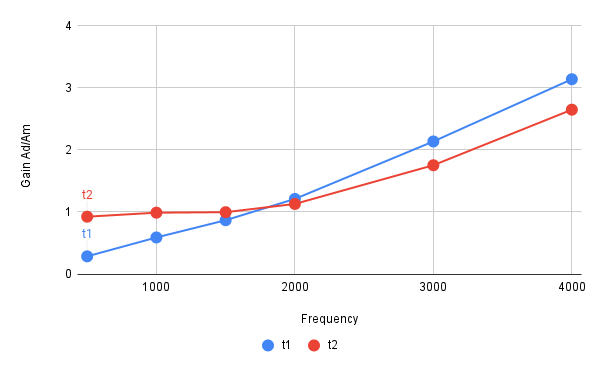
\includegraphics[width=0.7\textwidth]{assets/chart_1.png}
    \caption{$\tau_1$ vs $\tau_2$ without pre-emphasis}
\end{figure}
We notice that the loop filter $\tau_2$ is less sensitive to the message frequency than $\tau_1$, this is because $\tau_2$ has a lower cut-off frequency than $\tau_1$.
\begin{table}[H]
    \centering
    \begin{tabular}{|r|r|r|}
    \cline{1-3}
    \multicolumn{1}{|l|}{Freqeuncy} & \multicolumn{1}{l|}{$A_D$ using $\tau_1$} & \multicolumn{1}{l|}{$A_D$ using $\tau_2$} \\
    \cline{1-3}
    500  & 11.55 & 3.56 \\
    1000 & 8.87  & 5.27 \\
    1500 & 7.31  & 6.36 \\
    2000 & 5.94  & 6.37 \\
    3000 & 3.61  & 4.39 \\
    4000 & 2.44  & 2.9  \\
    \cline{1-3}
    \end{tabular}
    \caption{Amplitude Values without Pre-emphasis}
\end{table}
\begin{figure}[H]
    \centering
    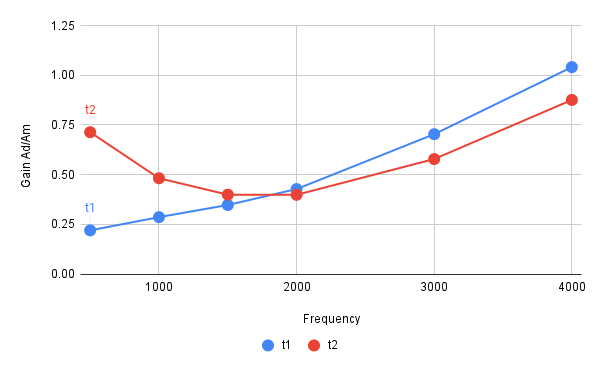
\includegraphics[width=0.7\textwidth]{assets/chart_2.png}
    \caption{$\tau_1$ vs $\tau_2$ with pre-emphasis}
\end{figure}
after using the pre-emphasis filter, we notice that the amplitude of the demodulated signal is higher than before, this is because the pre-emphasis filter amplifies the high-frequency portion of the signal, which improves the signal-to-noise ratio of the high-frequency portion of the baseband.
\begin{figure}[H]
    \centering
    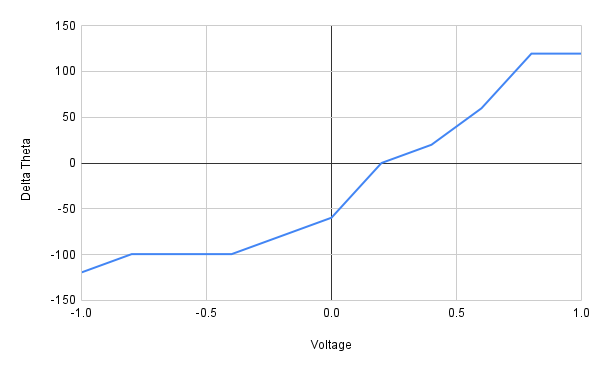
\includegraphics[width=0.7\textwidth]{assets/ch.png}
    \caption{$\tau_1$ with pre-emphasis vs $\tau_1$ without pre-emphasis}
\end{figure}
\begin{figure}[H]
    \centering
    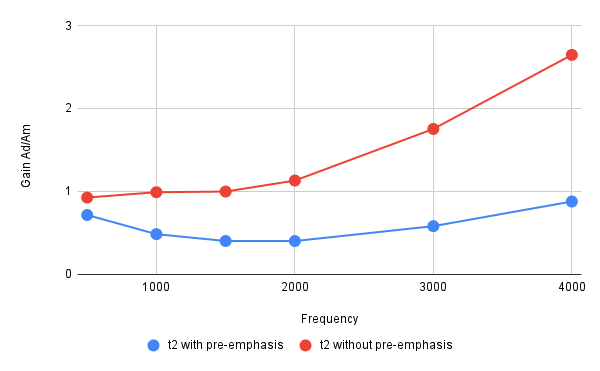
\includegraphics[width=0.7\textwidth]{assets/chart_5.png}
    \caption{$\tau_2$ with pre-emphasis vs $\tau_2$ without pre-emphasis}
\end{figure}
The pre-emphasis helps in equalizing the message signal power in terms of deviation ratio. Without pre-emphasis, the received audio would sound unacceptably noisy at high frequencies, especially under conditions of low carrier-to-noise ratio. Pre-emphasis increases the magnitude of the higher signal frequencies, thereby improving the signal-to-noise ratio.
\clearpage
\h{Conclusion}
In summary, this report illustrates the process of modulating and demodulating FM signals and studied the effect of different parameters such as message frequency, type, amplitude, carrier zeroing, pre-emphasis, and more. The use of pre-emphasis has been shown to improve the signal-to-noise ratio of the high-frequency portion of the baseband.
\clearpage
\bib{ref}
\end{document}





